% MSc dissertation example file, February 2022
%
% Leave one of the documentclass lines uncommented to match your degree.
% You may remove the logo option if it causes problems.
% Do not change any other options.
% \documentclass[logo,msc,adi]{infthesis}     % Adv Design Inf
% \documentclass[logo,msc,ai]{infthesis}      % AI
% \documentclass[logo,msc,cogsci]{infthesis}  % Cognitive Sci
% \documentclass[logo,msc,cs]{infthesis}      % Computer Sci
% \documentclass[logo,msc,cyber]{infthesis}   % Cyber Sec
% \documentclass[logo,msc,datasci]{infthesis} % Data Sci
% \documentclass[logo,msc,di]{infthesis}      % Design Inf
% \documentclass[logo,msc,dsti]{infthesis}    % Data Sci TI
% \documentclass[logo,msc,inf]{infthesis}     % Informatics
\documentclass[logo,msc]{infthesis}           % degree unspecified, do not change except to add your degree
%%%%%%%%%%%%%%%%%%%%%%%%
% Understand any problems and seek approval before assuming it's ok to remove ugcheck.
\usepackage{msccheck}

% Include any packages you need below, but don't include any that change the page
% layout or style of the dissertation. By including the ugcheck package above,
% you should catch most accidental changes of page layout though.

\usepackage{microtype} % recommended, but you can remove if it causes problems
\usepackage{graphicx}
\usepackage{subfig}

\begin{document}
\begin{preliminary}

\title{Machine Learning of Polyhedral Compilation}

\author{Prakshal Nandi}

\date{\today}

\abstract{
In most compute-intensive applications, a significant amount of time is spent on the execution of the loops. Compilers like clang offer many optimisation options such as loop tiling, unrolling, vectorization or parallel processing. Most optimizations are still particular to the loop they are trying to transform and require specific knowledge in this domain. If the loops follow a specific structure, it is possible to change the execution order of the loop statements to make the program run faster. But finding a profitable schedule at the compile time is a complex task, as there are lots of constraints and dependencies involved.

Fortunately, using the OpenAI Gym interface, PolyGym has converted this problem into an environment of optimizations for Reinforcement Learning algorithms. The loops are converted into polyhedral representation, upon which different transformations can be applied. This thesis explores the feasibility of using a Reinforcement Learning agent to find a profitable schedule. First, we generate valid schedules using agent-chosen actions transforming the polyhedral model. Secondly, we are doing a search in the space of the possible schedule to find the optimal solution using a different RL agent. Finally, with the help of some experiments, we show how different RL algorithms perform, starting from basic Q-Learning algorithm to more advanced and popular deep reinforcement learning algorithms.
}

\maketitle

\newenvironment{ethics}
   {\begin{frontenv}{Research Ethics Approval}{\LARGE}}
   {\end{frontenv}\newpage}

\begin{ethics}
This research does not involve any human participants or personal data. All data are collected based on simulation experiments on benchmark suites; hence no ethical concerns are associated with the project.

\standarddeclaration
\end{ethics}


\begin{acknowledgements}
Any acknowledgements go here.
\end{acknowledgements}


\tableofcontents
\end{preliminary}


\chapter{Introduction}

\section{Motivation}

Reinforcement Learning(RL) has recently been seen as a promising approach for compiler optimization \cite{8357388}\cite{9232934}. A Reinforcement Learning agent makes the \textit{observations} within the \textit{environment}, and takes \textit{actions} to receive certain \textit{rewards}. The goal is to maximize the rewards over a period of time. On the other side, to achieve optimizations related to data locality, memory management, communication, and automatic parallelization, the space of the possible transformations available to a compiler is vast. Applying Machine Learning(ML) algorithms to find a good strategy in this space is challenging. Polyhedral Compilation is one type of compiler optimization technique applicable to a particular class of nested loops. It can explore geometric dependency properties of kernel statements in different iterations and apply transformations to improve the schedule of the loop execution. In compiler optimization, machine learning is yet to achieve the level of success in other fields such as Computer Vision or Natural Language Processing. Even though it has been an object of research for more than two decades, machine learning guided techniques are still not widely utilized in industrial compilers.



\section{Objectives}

The aim of the project is to analyze how Reinforcement Learning can help improve Polyhedral Compilation. This analysis will be performed with the help of Deep Neural Networks and other hybrid meta-heuristics. The research hypothesis is that Reinforcement Learning algorithms can be generalized to learn Polyhedral Compilation.

It is not always clear how to represent the actual problem in a Reinforcement Learning environment. However, this part has already been covered in Polygym\cite{9563041}; hence it is not going to be the focus of this research. The main objectives for this project are trying to find answers to these questions:
\begin{itemize}

    \item Can we implement a Deep Reinforcement Learning algorithm that can help select the best actions related to polyhedral transformations? 
    \item Can we design reward functions that improve the training performance to learn profitable schedules?
    \item Can we explore different RL algorithms and find the most suitable technique by evaluating their performance?


\end{itemize}

\section{Structure}

This project proposal is structured as follows: Following the discussion regarding the problem statement, research objective, novelty, and significance of the project in Section 1, Section 2 provides an overview of the background and literature review. Section 3 focuses on project methodology, limitations, risks, and ethical considerations. Section 4 explains how the evaluation of the developed methods will be carried out. Section 5 discusses expected outcomes, and Section 6 outlines the research timeline, milestones, and deliverables.

\chapter{Background}

\section{Polyhedral Compilation}

The iteration space of a nested loop can be represented as an n-dimensional geometric model called a polytope. The optimization through Polyhedral Compilation is achieved in three different stages, moving from code to polyhedron model, applying program transformations within the model, and finally regenerating the code from the model. This model gives the framework to transform the loops, where the array references and loop bounds are affine functions of loop iterators and parameters. The polyhedral model is broadly applicable due to the high presence of affine loops in compute-bound applications\cite{poly_applicable}. In the kernel example shown in Figure 1, geometric interpretations such as two-dimensional polygons can be used to visualize dependencies between statements. Based on these dependencies, conclusions can be made regarding the preferred execution time of each statement. 

\section{Deep Reinforcement Learning}

The problem of reinforcement learning can become challenging if the number of states possible in the environment is too vast. Deep Learning addresses this challenge by approximating the Q-values of the state and action pairs, using model parameters called weights. The framework of deep learning is made of the neural network, consisting of an input layer, an output layer and one or more intermediate layers. The neurons in the layer have weights associated with 
them, which we are trying to optimize. The output generated by the network is compared with the target, and loss will be calculated. Different loss functions are available for comparisons, such as mean square error, cross-entropy loss or maximum likelihood loss. They all represent how far is the output of the model with respect to the desired result. Once we know the loss value, the gradients can be calculated considering the effect of each parameter on the output. Using an optimizer, such as SGD, Adam, or RMSprop, we can change the weight values to reduce the loss using the calculated gradients. We are moving towards the desired result by doing this in an iterative manner. Performing all these steps manually could be useful in understanding how deep learning works, but it could be extremely difficult in practical application. Luckily, we have libraries such as PyTorch available, which can calculate the gradients and perform backpropagation (may be more) to develop new network parameters.

\section{PyTorch}

PyTorch implements a dynamic graph approach for gradient calculation, where the library keeps track of the operations performed on the data, and unrolls this operation sequence when we need to calculate the associated gradients. The basic building block of DL is the \textit{tensor}, representing a multi-dimensional array, which is also implemented by this toolkit. PyTorch has methods to create tensors, convert numpy arrays to tensors, and generate tensors with specific data, such as \textit{torch.ones()}. It can also apply different operations on the tensors to concatenate, resize and transpose them. The library also allows for offloading the tensor calculations to GPU by specific the \textit{}device property associated with it. A tensor may or may not have gradient construction available to it, which can be configured and retrieved using properties such as \textit{requires\_grad} and \textit{grad}. By using \textit{backward} operation, we can ask PyTorch to calculate the gradients of all the variables in the network. By leveraging \textit{nn.Module} of PyTorch, we can define the network architecture, design dropouts, reinitiate the gradients and apply transformations such as \textit{Softmax} (may be more).

\section{PolyGym}

PolyGym provides an environment of Polyhedral optimizations for Reinforcement Learning, adhering to OpenAI Gym interface \cite{Gym}, which is a toolkit for solving RL problems. Suppose the actions are chosen to directly represent the transformations, such as loop fusion or tiling. In that case, the model may learn the profitable schedules only for a particular set of loops or domains. Instead, PolyGym takes a more granular approach\footnote{https://github.com/PolyGym/polygym}. It uses the existing formulation of Farkas' lemma from discrete geometry to construct the space of valid schedules. In the next step, a Markov decision process(MDP) can explore this space to find a profitable schedule, independent of the loop being optimized. Hence, this makes it a two-stage technique, the construction of schedule space and its exploration, using two different Markov Decision Processes with different states and actions. This framework, however, still lacks a training agent, although just by using this simple heuristic, PolyGym is able to find transformations that lead to a speed up of 3.39x over LLVM Or and 1.34x over best isl transformation \cite{9563041}. As shown in Figure 2, it should be noted that PolyGym does not use any agent, but an agent can use the environment defined by PolyGym for learning.

\section{Literature Review}

Previous surveys have explored the relationship between Machine Learning and Compiler Optimizations \cite{8357388}\cite{9232934}. Several studies have also begun to examine how RL can be applied to the field of compiler optimizations. In 2014, Emani \textit{et al.} demonstrated a new approach for dynamically mapping parallel programs to varying system resources \cite{10.1007}. They used Markov Decision Process for online thread scheduling and an offline model trained based on the system environment and the structure of the code. Similar to PolyGym, CompilerGym extends the Gym interface to provide a reinforcement learning environment to researchers for compiler optimizations \cite{CompilerGym}. A recent study by Mammadli \textit{et al.} presented an excellent example of using Deep Reinforcement Learning for finding effective sequences of phase-ordering, which is a long-standing problem for compiler generators \cite{static.neural}. However, finding profitable loop transformations is a much more fine-drawn problem than finding the optimum number of threads or distributing the work on different cores. In an investigation related to current Single Instruction, Multiple Data (SIMD) architectures, Neurovectorizer \cite{NeuroVectorizer} addresses the challenge to find a good vectorization strategy with the help of Deep Reinforcement Learning. MLGO \cite{10.48550} attempted to leverage Reinforcement Learning and Evolutionary Algorithms for making decisions about function in-lining for improving code size. However, the evaluation for the code size could be less challenging than the evaluation of the heuristics focusing on the program's execution speed due to the uncertainty involved in the time taken during each execution.

All these methods, however, did not consider polyhedral optimizations. In 1993, Feautrier presented the theoretical basis of the polyhedral formulation for single and multidimensional schedules \cite{single}\cite{multi}. After more than twenty years, Pouchet \textit{et al.} proposed an iterative optimization method for systematic exploration of the schedule search space \cite{it_Single}\cite{it_multi}. Building on top of these methods, Ganser \textit{et al.} demonstrated improvements in optimization with the use of genetic algorithms in 2017 \cite{10.1145/3109482}. One year later, they showed a reduction in benchmarking efforts by using surrogate performance models, where they trained the models based on the program transformation evaluated in the previous iterative optimizations, at the cost of 15\% degradation in speed-up \cite{10.1145/3291773}. This set of methods followed the iterative approach with benchmarking, making them time-consuming. In contrast, methods such as isl\cite{isl} and Pluto\cite{Bondhugula07pluto:a} generated the models directly to find a good compilation strategy in less time. However, this approach has certain limitations. The optimization performed is still dependent on the type of loop being analyzed, and its performance can not beat the time taking iterative methods. Hence, the proposed research with Reinforcement Learning fits very well between these two approaches.

\chapter{Methodology}

\section{Clang/LLVM/Polly}

LLVM is a set of optimiser libraries built around an intermediate representation of the code, known as LLVM-IR. Like many other analyzing and optimizing tools, it uses the Clang frontend, a \textit{C} language family compiler, as a library.
Polly applies polyhedral transformations on top of this intermediate representation. It first identifies relevant regions of the code suitable for transformations, called Static Control Parts(\textit{SCoP}). It then transforms these regions into a polyhedral representation based on integer sets and maps. On this representation, it applies optimisations, for example, related to data locality and parallelism, finally converting it back into the optimised version of the executable code. As Polly analyses the low-level IR instead of the programming language itself, it is not dependent on any language or platform.

A \textit{SCoP}, generally consisting of loops and conditions, contains part of the program for which control flow and memory access can be determined at the compile time. For a loop to be identified as \textit{SCoP}, the scalar expression for the iteration count should be able to be represented as an affine function. Similarly, the memory accesses for loading and storing should also be possible to be translated into an affine expression. Polly allows the export of this polyhedral representation into a \textit{JSON} based format called \textit{jSCoP}.
This allows us to apply external optimization, which can be imported back using the same \textit{jSCoP} format.

 Figure \ref{fig:Original_Loop} showcases an example of a \textit{C} loop doing matrix multiplication. Using \textit{clang}, we can identify the \textit{SCoP} parts of the code and convert them into LLVM representation as displayed in Figure \ref{fig:Poly_Rep}. The representation consists of statements as basic building blocks. Apart from its name, a \textit{statement} consists of \textit{Domain}, \textit{Schedule} and \textit{Access}. The \textit{domain} represents a set of different loop iterations executing the statement, as a named integer set. The \textit{schedule} is an integer map which assigns a point to each iteration in a multi-dimensional space following lexicographical order. Changing the schedule will change the order in which the kernel is executed. \textit{Access} is a pair of kind and relation. The kind can be either \textit{read}, \textit{write} or may \textit{write}. The access relation maps the domain with the memory space, which generally can be represented by an affine function. Figure \ref{fig:Dependencies} explains the dependencies information extracted from the above representation, which can exist between two statements or two iterations of the same statement. When the transformations have been applied, AST can be generated from the LLVM representation as shown in Figure \ref{fig:AST} and the program can be executed.

 \section{Q-learning}

 (improve this) The value of a state can be defined as the expectation of the maximum reward which can be gained from that state, considering all the actions that can be taken in that state. To select the optimal actions, we will need to determine the values of each action and select the one with the best possible result. In a way, the value of a state corresponds to the value of the action we can take from this state, giving us the maximum possible outcome.

 The state-action value can be represented as mentioned in Equation \ref{eq:SAQV} (change this),

\begin{equation}
Q(s,a) = r(s,a) + {\gamma} max_{a'\in A} Q(s',a')
\label{eq:SAQV}
\end{equation}
 
 A Q-Network can be trained by minimising the loss function at each iteration as shown in Equation \ref{eq:DQN} (change this),

\begin{equation} L_{i}(\theta _{i}) = E_{s,a\sim\rho(\cdot)}[(y_{i} - Q(s,a;\theta _{i}))^2]
\label{eq:DQN}
\end{equation}

where \(y_{i} = E_{s'\sim\epsilon}[r+\gamma\max\limits_{{a'}}Q(s', a'; \theta_{i-1})|s, a]]\) is the target for iteration i. \(\rho(s,a)\) is the probablity distribution over states s and actions a. \(\gamma\) is the discount factor, r is the reward, and \(Q(s,a;\theta)\) is the function approximator to estimate the action-value function \cite{DBLP:journals/corr/MnihKSGAWR13}.

\section{Agent Representation}

For the problems such as this, it is essential that the representation of the state is such that the agent is able to learn. We define two different agents here, one for the construction phase and one for the exploration. This is because the learning of the agent and the representation is completely different in both phases.

For the construction phase, the action space consists of three actions as defined in Equation \ref{eq:CONST_ACT},
\begin{equation}
A_{con} = \{next\_dimension, \hspace{1} select\_dependency, \hspace{1} next\_dependency\}
\label{eq:CONST_ACT}
\end{equation}

(add more explanation for actions)

The states during this phase represents information of dependecies with respect to the current dimension and it can be described as Equestion \ref{eq:CONST_SPC}

\begin{equation}
S_{con} = (i_{dim} ;\hspace{2} i_{dep};\hspace{2} d_{1i};\hspace{2} d_{1j};\hspace{2} d_{1k};\hspace{2} d_{2i};\hspace{2} d_{2j};\hspace{2} d_{2k};\hspace{2} n_d,\hspace{2} n_a)
\label{eq:CONST_SPC}
\end{equation}

In this representation, \textit{i\textsubscript{dim}} represents the current dimension, and \textit{i\textsubscript{dep}} represents the current dependency pointer. \textit{d\textsubscript{1i,1j,1k}} are related to loop variables of the first statement of the dependency and \textit{d\textsubscript{2i,2j,2k}} are variables for the second statements. We currently consider SCOP having a maximum of three iteration variables. \textit{n\textsubscript{d}} stores the number of strong dependencies added in current dimensions, and \textit{n\textsubscript{a}}
represents the number of total available dependencies.

\begin{figure}[!tb]
  \centering
  \subfloat[Original Loop in C.]{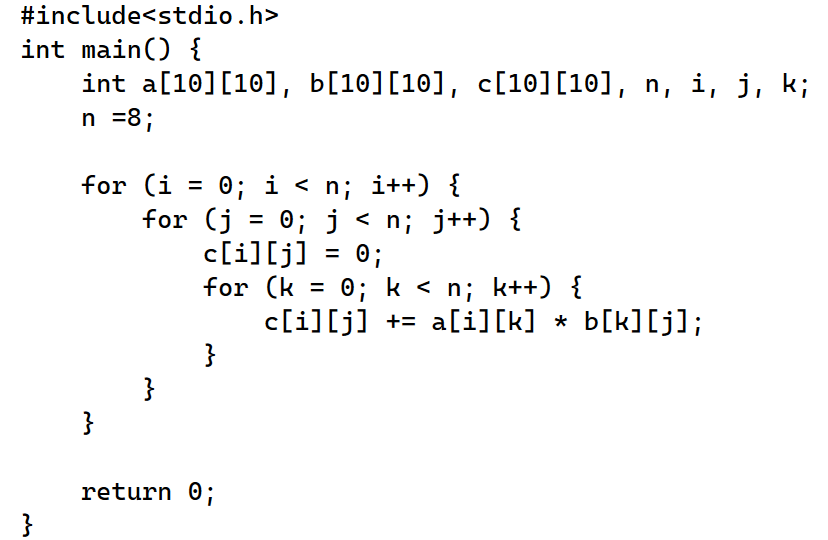
\includegraphics[width=0.5\textwidth]{Original_Loop.png}\label{fig:Original_Loop}}
  \hfill
  \subfloat[Polyhedral Representation of the identified SCoP.]{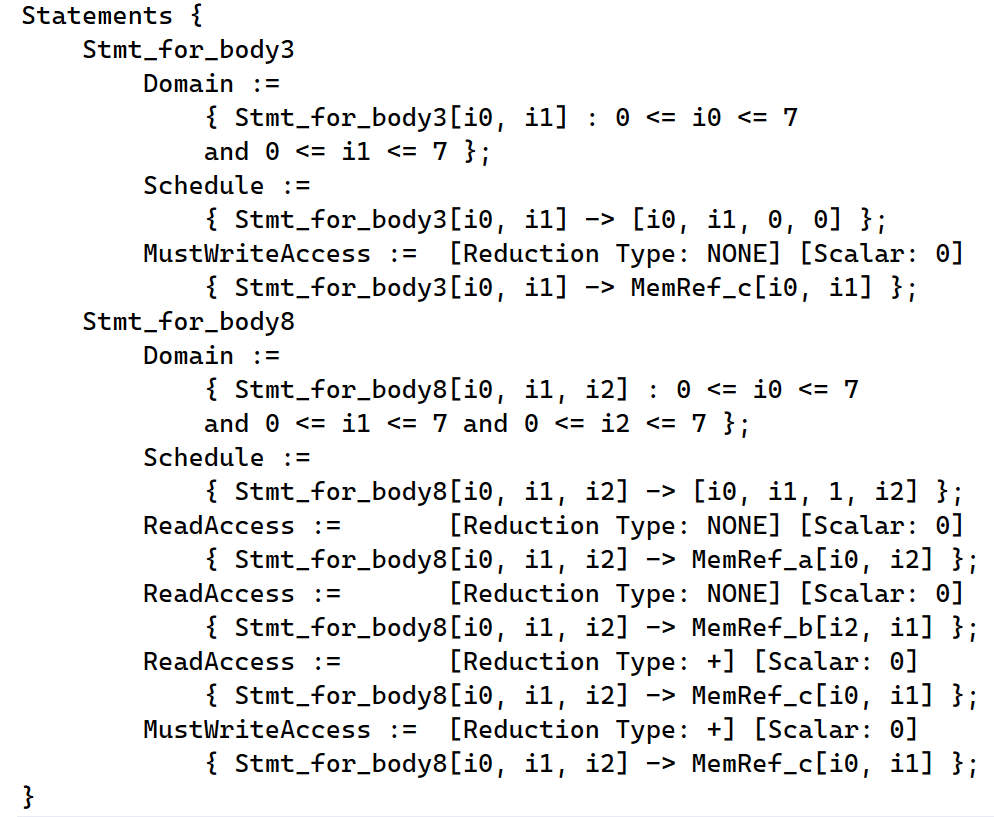
\includegraphics[width=0.5\textwidth]{Poly_Rep.png}\label{fig:Poly_Rep}}

  \centering
  \subfloat[Dependency Analysis.]{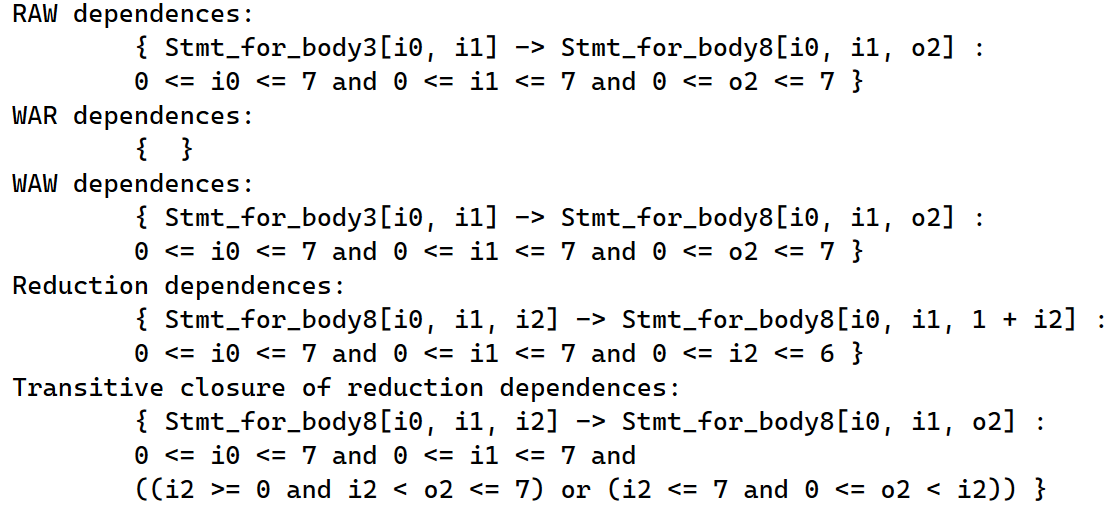
\includegraphics[width=0.5\textwidth]{Dependencies.png}\label{fig:Dependencies}}
  \hfill
  \subfloat[AST Generation from IR.]{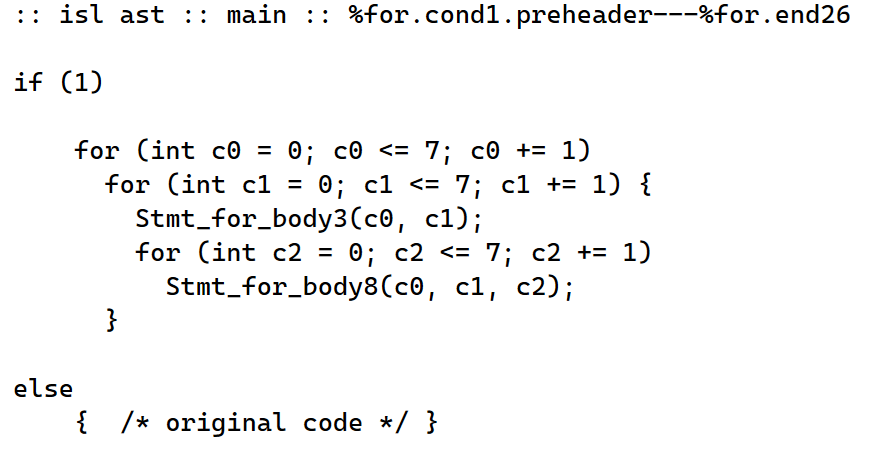
\includegraphics[width=0.5\textwidth]{AST.png}\label{fig:AST}}
  
  \caption{Generation of SCoP and AST using LLVM Polly}
\end{figure}


\chapter{Evaluation}

\chapter{Results and Discussions}

\chapter{Conclusions}

\section{Unresolved Issues}

\section{Future Work}

\bibliographystyle{plain}
\bibliography{mybibfile}


% You may delete everything from \appendix up to \end{document} if you don't need it.
\appendix

\chapter{First appendix}

\section{First section}





\end{document}
